%%
%% FGCS submission — cas-dc double-column format
%%
\PassOptionsToPackage{hyperfootnotes=false,hypertexnames=false}{hyperref}
\documentclass[a4paper,fleqn]{cas-dc}

\usepackage[numbers]{natbib}
\usepackage{amsmath,amssymb}
\usepackage{booktabs}
\usepackage{tabularx}
\usepackage{multirow}
\usepackage{array}
\usepackage{algorithm}
\usepackage{algorithmicx}
\usepackage{algpseudocode}
\usepackage{listings}
\usepackage{xcolor}
\usepackage{tikz}
\usetikzlibrary{positioning,arrows.meta,shapes,calc,shadows,fit}
\usepackage{pgfplots}
\pgfplotsset{compat=1.18}
\usepackage{float}
\usepackage{pifont}

\emergencystretch=3em
\hbadness=10000

\lstset{
  basicstyle=\ttfamily\scriptsize,
  breaklines=true,
  columns=fullflexible,
  frame=single,
  numbers=none,
  keywordstyle=\color{blue},
  commentstyle=\color{gray},
}

\providecommand{\doi}[1]{\url{https://doi.org/#1}}

\begin{document}
\let\WriteBookmarks\relax
\def\floatpagepagefraction{1}
\def\textpagefraction{.001}

\shorttitle{Decentralized Access Control for Agricultural Edge}
\shortauthors{Forcha et~al.}

\title[mode=title]{A Decentralized Hierarchical Role-Based Access
  Control Framework for Agricultural Edge Internet of Things: Design,
  Implementation, and 61-Day Field Evaluation}

\tnotemark[1]
\tnotetext[1]{The 61-day trace dataset, source code, deployment
  scripts, and chaincode supporting the findings of this study are
  publicly available at \url{https://github.com/forchag/blockchain-fet}.}

\author[1]{Forcha Glen Beloa}[orcid=0009-0003-1972-6100]
\cormark[1]
\ead{glenbeloa@gmail.com}
\credit{Conceptualization, Methodology, Software, Investigation,
  Writing -- Original Draft}

\affiliation[1]{organization={Department of Computer Engineering,
  Faculty of Engineering and Technology},
  city={Buea},
  country={Cameroon}}

\author[1]{Michael Ekonde Sone}
\ead{ekonde.sone@gmail.com}
\credit{Validation, Formal Analysis, Writing -- Review \& Editing}

\author[1]{Elie Fute Tagne}
\ead{eliefute@yahoo.fr}
\credit{Resources, Supervision, Writing -- Review \& Editing}

\author[2]{Andr\'{e} Paul Mvogo Asse}
\ead{mvogoasseandre@gmail.com}
\credit{Data Curation, Writing -- Review \& Editing}

\affiliation[2]{organization={\'{E}cole Nationale Sup\'{e}rieure
  Polytechnique de Douala, Universit\'{e} de Douala},
  city={Douala},
  country={Cameroon}}

\cortext[1]{Corresponding author}

\begin{abstract}
Agricultural Internet of Things (IoT) deployments involve stakeholder classes with
fundamentally incompatible access needs: a certification auditor
must read tamper-evident compliance logs without seeing real-time
irrigation commands, and a seasonal worker must actuate equipment in
one farm zone without querying sensor data from another. Centralizing
these decisions in a single server hands an attacker full operational
control the moment that server is compromised; it also leaves audit
logs mutable and delays credential revocation by days. This paper presents a
hierarchical role-based access control (HRBAC) framework on Hyperledger
Fabric~2.5 that distributes access-control enforcement across 64-bit
ARM (ARM64) edge nodes. A seven-role
hierarchy with zone and temporal constraints is provisioned through a
three-stage cascading enrollment protocol that operates under
intermittent long-range (LoRa) connectivity: the Certificate
Authority (CA) delegates
registration to Raspberry Pi~4B zone gateways, which provision
ESP32 sensor nodes using Ed25519 keys stored in one-time-programmable
eFuse. A 61-day deployment on an operational farm in Sfax, Tunisia
(50~sensors, 4~gateways, 146\,400~sensor-write transactions,
ambient temperatures reaching 39.5\textdegree{}C) yields 320\,ms
role-based access control (RBAC) overhead per sensor write,
63~transactions per second (TPS) at the
50-client benchmark scale, and 99.4\% uptime. Security tests ran 1\,000 automated attempts per vector across
eight testable vectors, blocking all 8\,000. When livestock
damaged a North-zone sensor on Day~34, certificate revocation
propagated to all peers within four hours and blocked 47~subsequent
access attempts while two supply-chain partners retained uninterrupted
read-only access.
\end{abstract}



\begin{graphicalabstract}
\centering
\resizebox{0.96\textwidth}{!}{%
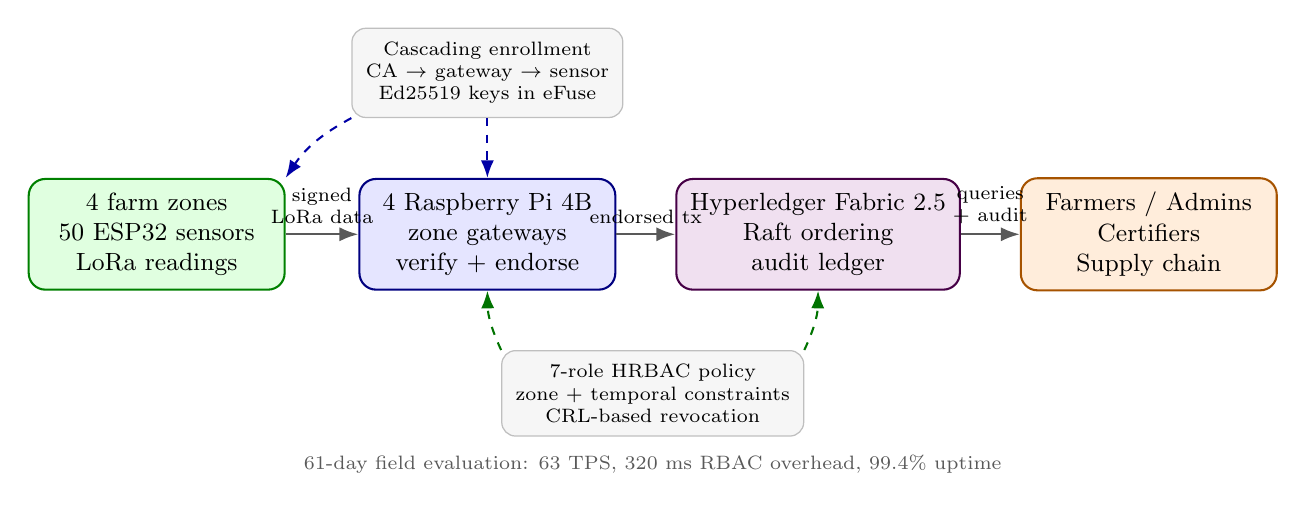
\begin{tikzpicture}[
    font=\small,>=Latex,
    component/.style={draw,rounded corners=6pt,minimum width=3.25cm,
      minimum height=1.28cm,align=center,line width=0.75pt,
      inner sep=5pt},
    sensor/.style={component,fill=green!12,draw=green!50!black},
    gateway/.style={component,fill=blue!10,draw=blue!50!black},
    ledger/.style={component,fill=violet!12,draw=violet!55!black},
    stakeholder/.style={component,fill=orange!14,draw=orange!65!black},
    note/.style={draw,rounded corners=5pt,fill=gray!7,draw=black!25,
      align=center,font=\scriptsize,inner sep=5pt,line width=0.45pt},
    flow/.style={->,line width=0.85pt,draw=black!65},
    enroll/.style={->,line width=0.75pt,draw=blue!65!black,dashed},
    policy/.style={->,line width=0.75pt,draw=green!45!black,dashed}
]
\node[sensor]      (sensors) at (0,2.2)
  {4 farm zones\\50 ESP32 sensors\\LoRa readings};
\node[gateway]     (gateways) at (4.2,2.2)
  {4 Raspberry Pi~4B\\zone gateways\\verify + endorse};
\node[ledger]      (fabric) at (8.4,2.2)
  {Hyperledger Fabric~2.5\\Raft ordering\\audit ledger};
\node[stakeholder] (users) at (12.6,2.2)
  {Farmers / Admins\\Certifiers\\Supply chain};

\draw[flow] (sensors) -- node[above,font=\scriptsize,align=center]
  {signed\\LoRa data} (gateways);
\draw[flow] (gateways) -- node[above,font=\scriptsize]{endorsed tx} (fabric);
\draw[flow] (fabric) -- node[above,font=\scriptsize,align=center]
  {queries\\+ audit} (users);

\node[note] (enroll) at (4.2,4.25)
  {Cascading enrollment\\CA $\rightarrow$ gateway $\rightarrow$ sensor\\Ed25519 keys in eFuse};
\node[note] (policy) at (6.3,0.18)
  {7-role HRBAC policy\\zone + temporal constraints\\CRL-based revocation};

\draw[enroll] (enroll.south west) to[bend right=14] (sensors.north east);
\draw[enroll] (enroll.south) -- (gateways.north);
\draw[policy] (policy.north west) to[bend left=12] (gateways.south);
\draw[policy] (policy.north east) to[bend right=12] (fabric.south);

\node[font=\scriptsize,text=black!65,align=center] at (6.3,-0.72)
  {61-day field evaluation: 63 TPS, 320 ms RBAC overhead, 99.4\% uptime};
\end{tikzpicture}}
\end{graphicalabstract}

\begin{highlights}
\item Seven-role HRBAC on Hyperledger Fabric, zone and temporal
  constraints, TLA+ verified (5\,184 states).
\item Cascading enrollment for 520\,KB ESP32 sensors under intermittent
  LoRa: Ed25519 in eFuse, TPM~2.0 gateway keys.
\item 61-day field deployment: 63\,TPS, 320\,ms RBAC overhead,
  99.4\% uptime, 8\,000 security tests blocked.
\item Day~34 field incident: certificate revocation published
  within 60\,s, propagated to all peers in 4.2\,min, blocking
  47 subsequent attempts with zero disruption to other stakeholders.
\item CRT-based LoRa transmission cuts per-event sensor energy from
  24.21\,mJ to 12.40\,mJ via single-residue recovery.
\end{highlights}

\begin{keywords}
Hierarchical Role-Based Access Control \sep Hyperledger Fabric \sep
Agricultural IoT \sep Edge Computing \sep ARM64 Architecture \sep Certificate
Lifecycle Management \sep Blockchain Access Control
\end{keywords}

\maketitle

%%=============================================================
\section{Introduction}
\label{sec:intro}
%%=============================================================

A modern precision farm generates sensor readings from soil moisture
probes, weather stations, and irrigation actuators at rates that can
exceed several thousand transactions per day~\cite{zhang2002precision}.
Six distinct stakeholder classes interact with this data: farmers
requiring full operational control; agronomists needing read access to
historical records without equipment control; certification bodies
(organic, GlobalGAP) auditing compliance without seeing proprietary
agronomic practices; supply-chain partners accessing provenance data
without real-time operational visibility; extension services working
with anonymized datasets; and regulatory authorities verifying
environmental compliance records.

Conventional deployments handle this authorization matrix through a
single authentication server. Compromising that server grants an attacker
not just data access but
potentially full irrigation control~\cite{benedict2021decentralized},
and the mutable logs it maintains make post-incident forensics depend
on the integrity of whoever operates the server, a single point of trust
that blockchain-based architectures are designed to remove. Consistent
with the access-control gap identified by Ferrag et
al.~\cite{ferrag2020security}, deployed systems typically grant broad
read permissions to authenticated users, so a supply-chain auditor
querying shipment records can also read real-time soil nutrient data
that the farmer treats as proprietary.
Credential revocation lags behind the physical event by days, because
decommissioning a damaged sensor or terminating a seasonal worker's
access requires manual database edits on a timeline set by whoever is
monitoring the system~\cite{wang2006wireless,ferrag2020security}.

Ferrag et al.~\cite{ferrag2020security}, surveying agricultural IoT
deployments through 2019, found that 78\% lacked fine-grained access
control and only 23\% implemented cryptographic device identity. Kamilaris et al.~\cite{kamilaris2019rise}, reviewing blockchain
agriculture projects published through mid-2019, found that 87\%
targeted post-harvest supply-chain tracking, leaving pre-harvest
authorization as largely unaddressed ground.

\subsection{Limitations of Prior Blockchain-IoT Access Control}
\label{subsec:prior_limits}

Capability-token systems such as FairAccess~\cite{ouaddah2016fairaccess}
and BlendCAC~\cite{xu2018blendcac} address decentralized delegation but
not the role-stakeholder structure, geographic zones, or seasonal
expiration that agricultural deployments require. FairAccess maps grants
to Bitcoin-like transfers: ten-minute confirmation windows make it
unusable for irrigation control, and BlendCAC's ERC-721 tokens incur
per-transaction gas fees that are incompatible with sensor duty cycles.

Permissioned-platform work closes the latency problem. Shih et
al.~\cite{shih2022iiot} confirmed Fabric-based access control runs on
Raspberry Pi~4B ARM64 hardware; Pajooh et al.~\cite{pajooh2022fabric_iot}
and Ke and Park~\cite{kepark2023fabric_model} contributed testbed and
performance models. None report multi-week field deployment data.
Idrissi and Palmieri~\cite{idrissi2024blockchain_jsupercomput} provide
the only published end-to-end Fabric latency breakdown on constrained
ARM hardware, albeit in a healthcare context; their methodology informs
our benchmark design in Section~\ref{subsec:bench}. Usman et al.~\cite{usman2024blockchain} propose
smart-contract-enforced domain policies for industrial IoT using
cloud-hosted nodes that don't face the memory and thermal constraints of
outdoor ARM64 hardware. Zaidi et al.~\cite{zaidi2023fabrication} report
approximately 12\,s response time for 35 concurrent users in simulation;
our field deployment measures a P95 latency of 1.48\,s under comparable
concurrency, though their simulation does not specify equivalent hardware
or workload type; the gap would likely narrow under controlled comparison.

The gap is not only in policy design. An ESP32 sensor with 520\,KB
SRAM and intermittent LoRa connectivity cannot contact a remote CA
directly; measurements of lightweight secure IoT stacks show that TLS-style
handshakes can dominate constrained-device memory budgets~\cite{raza2013lithe},
and the mbedTLS handshake stack on ESP-IDF requires approximately
70\,KB of heap, leaving insufficient headroom for the sensor application
layer within the 520\,KB SRAM budget. Any design
that assumes pre-established device identities leaves the hardest
operational problem, secure enrollment through local gateways, outage
tolerance, and protected key storage, outside the published solution
space.

\subsection{Contributions}
\label{subsec:contributions}

This paper makes five contributions:

\begin{enumerate}
\item A seven-role HRBAC model with zone and temporal constraints,
  where role inheritance reduces the administrative overhead of the
  six-class agricultural stakeholder structure while preserving security
  boundaries between them (Section~\ref{sec:architecture}).

\item A three-stage cascading enrollment protocol that delegates CA
  privileges to zone gateways, which provision ESP32 nodes using
  Ed25519 key pairs stored in one-time-programmable eFuse; the
  protocol is designed and iteratively validated against the 6--18-hour
  gateway outages encountered in the field (Section~\ref{subsec:ops}).

\item A 61-day field deployment on an operational Tunisian farm
  yielding 320\,ms RBAC overhead, 63~TPS, 99.4\% uptime, and 100\%
  blocking across 8\,000 security tests against eight testable attack
  vectors (Sections~\ref{sec:evaluation}--\ref{sec:security}).

\item Partial formal verification of role-permission invariants in TLA+,
  with zone isolation and temporal expiration tested empirically
  (Section~\ref{sec:security}).

\item CRT-based LoRa transmission that reduces per-event sensor energy
  from 24.21\,mJ to 12.40\,mJ; three residues transmitted sequentially
  on separate channels give single-residue forward error recovery,
  letting the sensor lower transmit power on each channel
  (Section~\ref{sec:implementation}).
\end{enumerate}

%%=============================================================
\section{Related Work}
\label{sec:related}
%%=============================================================

\subsection{Access Control for the Internet of Things (IoT)}
\label{subsec:ac_iot}

The Role-Based Access Control (RBAC) model formalized by Sandhu
et al.~\cite{sandhu1996role} and standardized by the National
Institute of Standards and Technology (NIST) into Core, Hierarchical,
and Separation of Duty variants~\cite{ferraiolo2001role} remains the
baseline for multi-user authorization. Its Internet of Things (IoT)
extensions share a common assumption: some trusted decision component
must remain reachable when access is requested. RBAC extensions for
IoT~\cite{ye2015iot}, Attribute-Based Access Control (ABAC)
evaluation~\cite{hu2014guide,servos2017abac,sciancalepore2017oauth}, and Capability-Based
Access Control (CapBAC) token delegation~\cite{hernandez2017capability}
place that trust in a policy engine, an attribute authority, or a
credential issuer, respectively. Sciancalepore et al.~\cite{sciancalepore2017oauth}
show that open-standard authorization stacks still impose measurable
overhead on constrained IoT hardware, reinforcing the need to push
heavy policy evaluation to gateways or ledger peers rather than
sensors.

These designs reduce different parts of the problem but leave a
central dependency. Ye et al.~\cite{ye2015iot} and Servos and
Osborn~\cite{servos2017abac} retain a central enforcement point for
role or attribute evaluation. Hern\'{a}ndez-Ramos et
al.~\cite{hernandez2017capability} move authorization into tokens, but
revocation becomes distributed once those tokens have been issued.
Alshehri and Sandhu~\cite{alshehri2016access} split the model by
assigning RBAC to human users and CapBAC to devices, leaving the role
store as the remaining centralized dependency. Our framework removes
that dependency by storing role assignments, revocations, and zone
constraints as append-only ledger entries evaluated by chaincode.

\subsection{Blockchain-Based Access Control}
\label{subsec:blockchain_ac}

Table~\ref{tab:sota} positions our work against prior systems on the
two metrics most consequential for real-time IoT: throughput and
end-to-end latency. Here, N/R means not reported, N/A means not
applicable, and TPS means transactions per second.

\begin{table}[pos=t]
\caption{Throughput and latency: this work versus prior blockchain
  access control systems. N/R = not reported; N/A = not applicable.}
\label{tab:sota}
\resizebox{\tblwidth}{!}{%
\begin{tabular}{@{}lllll@{}}
\toprule
System & Platform & TPS & Latency & Deployment \\
\midrule
FairAccess~\cite{ouaddah2016fairaccess} & Bitcoin & 0.002 & 600\,000\,ms & N/A \\
BlendCAC~\cite{xu2018blendcac} & Ethereum & 15 & 3\,200\,ms & N/A \\
Zaidi et al.~\cite{zaidi2023fabrication} & Fabric & 0.08 & 12\,000\,ms & Simulation \\
Shih et al.~\cite{shih2022iiot} & Fabric & N/R & N/R & Lab \\
Idrissi \& Palmieri~\cite{idrissi2024blockchain_jsupercomput} & Fabric & N/R & See ref. & Lab \\
Putra et al.~\cite{putra2021trust} & Fabric & N/R & See ref. & Lab \\
\textbf{This work} & Fabric & \textbf{63} & \textbf{1\,220\,ms} & \textbf{61 days} \\
\bottomrule
\end{tabular}}
\end{table}

Table~\ref{tab:feature_comparison} adds the dimension that
throughput-latency comparisons miss: which architectural features each
system actually implements. A check mark indicates an implemented and
evaluated feature, a cross indicates absence, and \textit{Partial}
indicates partial implementation. Our framework is the only one in this set
that combines zone constraints, temporal permissions, cascading
enrollment for constrained devices, field-validated ARM64 deployment,
and certificate lifecycle management.

\begin{table*}[width=\textwidth,pos=t]
\caption{Feature comparison across blockchain-based access control
  systems. \ding{51} = implemented and evaluated;
  \ding{55} = absent; Partial = partially implemented.}
\label{tab:feature_comparison}
\small
\begin{tabularx}{\tblwidth}{@{}l
  >{\centering\arraybackslash}X
  >{\centering\arraybackslash}X
  >{\centering\arraybackslash}X
  >{\centering\arraybackslash}X
  >{\centering\arraybackslash}X
  >{\centering\arraybackslash}X
  >{\centering\arraybackslash}X@{}}
\toprule
System &
  Zone Const. &
  Temporal Perm. &
  Cascade Enroll. &
  ARM64 Field &
  Cert.\ Lifecycle &
  Formal Verif. &
  Deploy.\ Duration \\
\midrule
FairAccess~\cite{ouaddah2016fairaccess}   & \ding{55} & \ding{55} & \ding{55} & \ding{55} & Limited & \ding{55} & N/A \\
BlendCAC~\cite{xu2018blendcac}            & \ding{55} & \ding{55} & \ding{55} & \ding{55} & Limited & \ding{55} & N/A \\
Shih et al.~\cite{shih2022iiot}           & \ding{55} & \ding{55} & \ding{55} & Lab       & \ding{55} & \ding{55} & Days \\
Zaidi et al.~\cite{zaidi2023fabrication}  & \ding{55} & \ding{55} & \ding{55} & \ding{55} & \ding{55} & \ding{55} & Simulation \\
Usman et al.~\cite{usman2024blockchain}   & \ding{55} & \ding{55} & \ding{55} & \ding{55} & \ding{55} & \ding{55} & Days \\
Bandara et al.~\cite{bandara2021modeling} & \ding{55} & \ding{55} & \ding{55} & \ding{55} & \ding{55} & \ding{55} & Simulation \\
\textbf{This work}                        & \ding{51} & \ding{51} & \ding{51} & \ding{51} & \ding{51} & Partial   & 61 days \\
\bottomrule
\end{tabularx}
\end{table*}

Bandara et al.~\cite{bandara2021modeling} model IoT access control
policies for supply-chain traceability, but their work targets
post-harvest distribution rather than pre-harvest operations such as
zone-controlled irrigation and pesticide application. Liu et
al.~\cite{liu2019edge} and Wang et al.~\cite{wang2021edge} reduced
processing latency at the agricultural IoT edge without addressing the
authorization layer on top of that edge infrastructure.

On identity infrastructure, World Wide Web Consortium (W3C)
Decentralized Identifier (DID)~\cite{w3c_did_core} and
gateway-assisted DID verification for constrained devices~\cite{ferdous2019ssi}
offer
a migration path away from X.509. Tzenetopoulos et
al.~\cite{tzenetopoulos2022hlfkubed} established a performance floor
for Fabric on Raspberry Pi~3B+ ARM hardware: 448\,MB memory usage,
1.1\,s transaction latency. A peer-count-controlled reading is more
conservative: at 4~peers our P95 is 1,480\,ms, about 35\% higher than
Tzenetopoulos's 1,100\,ms figure for a Pi~3B+ without access-control
chaincode. At 32~peers the P95 falls to 855\,ms, about 22\% below their
figure, suggesting that additional peers plus the Pi~4B Cortex-A72 and
ARM64 Fabric stack provide the latency benefit.

%%=============================================================
\section{System Architecture}
\label{sec:architecture}
%%=============================================================

\subsection{Deployment Overview}
\label{subsec:overview}

Fifty ESP32-WROOM-32 sensors, four Raspberry Pi~4B gateways, and
an x86 Fabric backend form the three physical tiers of the deployment.
Sensor nodes (dual-core Xtensa LX6 @ 240\,MHz, 520\,KB SRAM) collect soil
moisture, temperature, and environmental data, sign each reading with
an Ed25519 key stored in one-time-programmable eFuse, and transmit
over LoRa radio at spreading factor~7 (SF7) and 125\,kHz bandwidth
(BW). Four Raspberry Pi~4B gateways
(quad-core Cortex-A72, 4\,GB low-power double data rate~4
(LPDDR4), Trusted Platform Module (TPM)\,2.0) receive sensor
payloads, verify signatures, endorse Fabric transactions, and cache
access policies locally. Gateways interconnect via a BATMAN-adv
mesh~\cite{batman2010} that reroutes traffic around individual gateway
failures without manual reconfiguration; the mesh also carries Fabric
gossip and Certificate Revocation List (CRL) update traffic between
zones. The Fabric network runs
three Raft orderers
(crash-fault tolerant (CFT), $f{=}1$) and four peer nodes (one per zone)
on x86 management hardware; CouchDB~3.2 handles world-state queries.
Figure~\ref{fig:enrollment} shows the three-stage cascading
enrollment protocol: Stage~1 issues administrator credentials, Stage~2
registers gateways, and Stage~3 provisions sensor certificates after
key generation and certificate signing request (CSR) submission.

\begin{figure}[pos=t]
\centering
\resizebox{\columnwidth}{!}{%
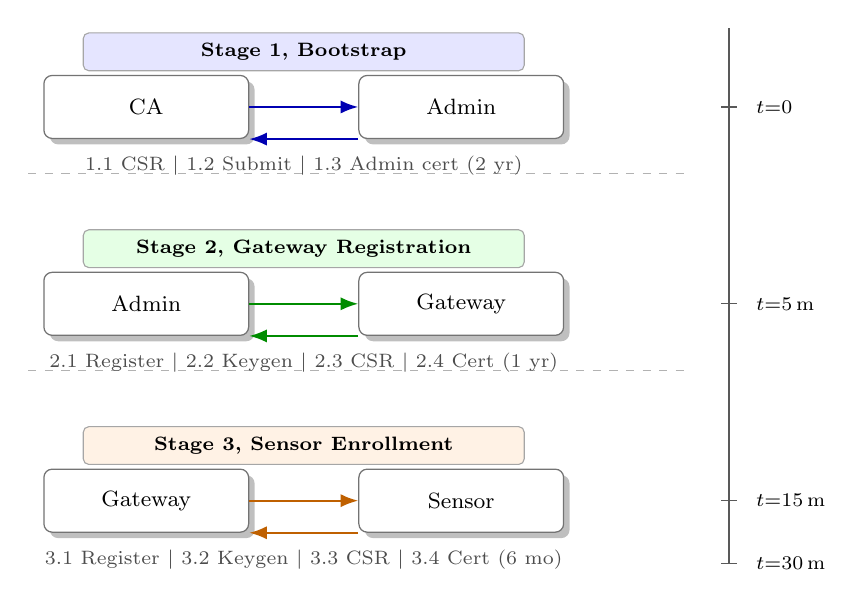
\begin{tikzpicture}[
    x=1cm, y=1cm, >=Latex, font=\footnotesize,
    entity/.style={draw, rounded corners=3pt, minimum width=2.6cm,
      minimum height=0.8cm, align=center, fill=white,
      line width=0.45pt, draw=black!55, drop shadow},
    stage/.style={draw, rounded corners=2pt, minimum width=5.6cm,
      minimum height=0.48cm, align=center,
      font=\scriptsize\bfseries, inner sep=2pt, draw=black!35},
    stepline/.style={font=\scriptsize, text=black!70},
    arr1/.style={->, line width=0.75pt, draw=blue!70!black},
    arr2/.style={->, line width=0.75pt, draw=green!55!black},
    arr3/.style={->, line width=0.75pt, draw=orange!75!black},
    tl/.style={line width=0.4pt, draw=black!65},
    sep/.style={line width=0.35pt, draw=black!30, dashed}
]
\node[stage, fill=blue!10]   at (3.8,7.6) {Stage 1, Bootstrap};
\node[stage, fill=green!10]  at (3.8,5.1) {Stage 2, Gateway Registration};
\node[stage, fill=orange!10] at (3.8,2.6) {Stage 3, Sensor Enrollment};
\draw[sep] (0.3,6.05) -- (8.7,6.05);
\draw[sep] (0.3,3.55) -- (8.7,3.55);
\node[entity] (ca1) at (1.8,6.9) {CA};
\node[entity] (ad1) at (5.8,6.9) {Admin};
\draw[arr1] (ca1.east) -- (ad1.west);
\draw[arr1] (ad1.south west) -- (ca1.south east);
\node[stepline] at (3.8,6.15)
  {1.1~CSR \textbar\ 1.2~Submit \textbar\ 1.3~Admin cert (2~yr)};
\node[entity] (ad2) at (1.8,4.4) {Admin};
\node[entity] (gw2) at (5.8,4.4) {Gateway};
\draw[arr2] (ad2.east) -- (gw2.west);
\draw[arr2] (gw2.south west) -- (ad2.south east);
\node[stepline] at (3.8,3.65)
  {2.1~Register \textbar\ 2.2~Keygen \textbar\ 2.3~CSR \textbar\ 2.4~Cert (1~yr)};
\node[entity] (gw3) at (1.8,1.9) {Gateway};
\node[entity] (sn3) at (5.8,1.9) {Sensor};
\draw[arr3] (gw3.east) -- (sn3.west);
\draw[arr3] (sn3.south west) -- (gw3.south east);
\node[stepline] at (3.8,1.15)
  {3.1~Register \textbar\ 3.2~Keygen \textbar\ 3.3~CSR \textbar\ 3.4~Cert (6~mo)};
\draw[tl] (9.2,1.1) -- (9.2,7.9);
\foreach \y/\lbl in {6.9/{$t{=}0$},4.4/{$t{=}5$\,m},
                      1.9/{$t{=}15$\,m},1.1/{$t{=}30$\,m}}{
  \draw[tl] (9.1,\y) -- (9.3,\y)
    node[right=0.12cm, font=\scriptsize] {\lbl};
}
\end{tikzpicture}}
\caption{Cascading enrollment protocol}
\label{fig:enrollment}
\end{figure}

\subsection{Threat Model}
\label{subsec:threat}

Fabric orderer nodes and Certificate Authorities are operated by vetted
institutional entities and treated as non-malicious, consistent with
the permissioned blockchain model in which all participants are
credentialed~\cite{androulaki2018fabric}. Raft provides crash-fault
tolerance with $2f{+}1$ nodes; our three-node cluster tolerates one
orderer failure but does not protect against a reachable node acting
maliciously~\cite{ongaro2014raft}. This Raft choice is therefore both a
throughput ceiling and a security-assumption boundary: stronger ordering
services such as HotStuff~\cite{yin2019hotstuff},
PBFT~\cite{castro1999practical}, or Fabric~v3.0's SmartBFT-based
ordering would raise the consensus cost but also move the system beyond
the present crash-fault-tolerant threat model.

Edge devices, end-user clients, and all wireless channels are treated
as potentially compromised. Four attack classes define the security
perimeter: unauthorized access via credential theft or replay;
privilege escalation through role-hierarchy vulnerabilities;
zone-boundary violations; and availability attacks through transaction
flooding. Physical tampering and side-channel attacks on cryptographic
accelerators are outside the current evaluation scope.

\subsection{Seven-Role HRBAC Model}
\label{subsec:rbac}

Following the formal treatment of hierarchical role administration in
ARBAC97~\cite{sandhu1999arbac97}, a partial order $\preceq$ over the role
set $R$ defines the role hierarchy,
where $r_i \preceq r_j$ iff $\mathrm{permissions}(r_i) \subseteq
\mathrm{permissions}(r_j)$. The inheritance relation separates the
operational chain from audit and supply-chain branches:
\begin{align}
\mathrm{Agronomist} &\preceq \mathrm{Farmer} \preceq \mathrm{Admin}
\label{eq:ops_chain}\\
\mathrm{Certifier} &\preceq \mathrm{Admin}, \quad
\mathrm{SupplyChain} \preceq \mathrm{Admin}
\label{eq:audit_supply_branches}\\
\mathrm{Sensor} &\preceq \mathrm{Gateway} \preceq \mathrm{Admin}
\label{eq:device_chain}
\end{align}
Admin holds all permissions; SupplyChain and Sensor are leaf roles with
the most restricted sets, and Certifier remains a separate audit branch
rather than a parent of Agronomist. The effective permissions of user $u$
in a session are:
\[
\mathrm{eff}(u) = \bigcup_{r \in \mathrm{active}(u)}
  \bigcup_{r' \preceq r} pa(r')
\]
where $pa(r)$ is the permission set directly assigned to role $r$ and
$\mathrm{active}(u)$ is the set of non-expired roles assigned to $u$.

An access request $(u, \mathit{op}, \mathit{res}, t)$ is granted iff:
\begin{equation}
\begin{aligned}
&\exists\, r \in \mathrm{active}(u,t):
  (\mathit{op},\mathit{res}) \in \mathrm{eff}(r) \\
&\quad{}\land\;
  \bigl(\mathrm{zone}(u)=\mathrm{zone}(\mathit{res})
  \lor \mathrm{czt}(u,\mathrm{zone}(\mathit{res}),t)\bigr)
\end{aligned}
\label{eq:access}
\end{equation}
where $\mathrm{czt}(u, z, t)$ is true iff $u$ holds a valid
administrator-issued cross-zone token for zone $z$ at time $t$.
Active roles are time-bounded:
$\mathrm{active}(u,t) = \{r \mid \exists\,\mathrm{assign}(u,r,t_s,t_e)
: t_s \le t \le t_e\}$.

Table~\ref{tab:permissions} shows the resulting permission matrix. In
the table, \textit{own} means own zone only, \textit{zone} means the
assigned zone, \textit{all} means all zones, and \textit{ctrl} denotes
control permission.

\begin{table*}[width=\textwidth,pos=t]
\caption{Permission matrix for agricultural resources across seven
  roles. \textit{own} = own zone only; \textit{zone} = assigned
  zone; \textit{all} = all zones.}
\label{tab:permissions}
\small
\begin{tabularx}{\tblwidth}{@{}l*{7}{>{\centering\arraybackslash}X}@{}}
\toprule
Resource & Sensor & Gateway & Farmer & Agron. & Cert. & Supply & Admin \\
\midrule
Sensor data       & own  & zone     & all      & all  & all  & N/A   & all  \\
Irrigation ctrl   & N/A  & zone     & full     & N/A  & N/A  & N/A   & full \\
Audit logs        & N/A  & N/A      & N/A      & N/A  & read & N/A   & full \\
Role assignments  & N/A  & N/A      & N/A      & N/A  & N/A  & N/A   & full \\
Cross-zone tokens & N/A  & N/A      & N/A      & N/A  & N/A  & N/A   & issue\\
\bottomrule
\end{tabularx}
\end{table*}

\subsection{Zone and Temporal Constraints}
\label{subsec:constraints}

Geographic farm regions (North, South, East, West) define the zone model
and are enforced at three levels. Each device certificate embeds the
zone attribute in the X.509 Subject Alternative Name extension under
OID \texttt{1.3.6.1.4.1.54392.1.2} with value format \texttt{Zone=North};
latitude, longitude, and radius fields follow under OIDs
\texttt{.3}--\texttt{.5}. Each gateway accepts CSRs only from sensors
whose declared zone matches its own. At the chaincode level, every
transaction accessing a zone-scoped resource calls
\texttt{validateZoneAccess}, which parses the caller's zone from the
certificate DER bytes using ASN.1 decoding, not PEM string
matching, and rejects the transaction if zones do not match and no
valid cross-zone token exists.

Cross-zone tokens are administrator-issued and stored immutably on the
ledger with user~ID, permitted zone list, validity period, and purpose
field. An agronomist with a North-zone certificate who needs to audit
South-zone data during a multi-farm review receives a time-bounded
token rather than a re-issued certificate.

Temporal constraints operate at two independent layers. The chaincode
checks an \texttt{ExpiresAt} timestamp in the \texttt{RoleAssignment}
structure against the Fabric transaction timestamp before every access
decision. The Fabric MSP independently validates the X.509
\texttt{NotAfter} field on every incoming transaction. A seasonal worker
assigned the \texttt{Farmer} role for 90~days during harvest is revoked
automatically at expiry; the revocation creates a new audit record
referencing the original assignment while both remain immutable on the
ledger.

Gateways carry u-blox NEO-M9N Global Positioning System (GPS) modules
whose one-pulse-per-second (1-PPS) signal provides sub-microsecond time
references at the gateway level. Network Time Protocol (NTP) distributes
this across the broader system at millisecond precision, well within
the $\pm$5-minute temporal enforcement window.

\subsection{Cascading Enrollment Protocol}
\label{subsec:enrollment}

An ESP32 with 520\,KB static random-access memory (SRAM) cannot hold
the Transport Layer Security (TLS) handshake stack that a direct
certificate authority (CA) interaction requires; this design follows the
constrained-device motivation established by lightweight secure CoAP/TLS
work~\cite{raza2013lithe}. The three-stage protocol in
Figure~\ref{fig:enrollment} delegates provisioning authority to zone
gateways. Stage~1 issues long-term admin credentials (2-year validity).
Stage~2 has the administrator register each gateway; the CA issues a
1-year zone-bound certificate, and the gateway stores its private key
in TPM~2.0 (Infineon SLB9670). In Stage~3, each gateway acts as a
local registration authority: the sensor generates an Ed25519 key pair,
writes the 32-byte private key to \texttt{EFUSE\_BLK\_KEY0}, calls
\texttt{esp\_efuse\_set\_read\_dis(EFUSE\_BLK\_KEY0)} to block
subsequent software reads, and sends a CSR to the gateway. The CA issues
a 6-month zone-bound certificate with the zone attribute embedded in
the Subject Alternative Name (SAN) extension.

CRL publication triggers immediately on an admin command, propagating
to all four peers via Fabric gossip (4.2~minutes average), and also
runs on a daily schedule. During the three connectivity outages of
6--18~hours each, peers operated on the most recently cached CRL
without error. A compromised certificate can therefore be reused for
up to 24~hours if the revocation event falls inside an outage window;
this is an accepted trade-off against the connectivity realities of
the deployment, and is documented as a residual risk in
the threat model.

\subsection{Execute-Order-Validate Flow}
\label{subsec:eov}

Figure~\ref{fig:eov} (cross-zone token, CZT, defined in
Section~\ref{subsec:constraints}) shows the Hyperledger Fabric
execute-order-validate flow with HRBAC checks at the endorsement stage.
Role activity, zone matching, Certificate Revocation List (CRL) lookup,
and nonce uniqueness are all checked before a transaction is forwarded
to the Raft orderer. A rejected transaction never reaches the ledger.
Figure~\ref{fig:eov} also marks the cross-zone token (CZT) path and
the multi-version concurrency control (MVCC) validation stage.

\begin{figure}[pos=t]
\centering
\resizebox{0.95\columnwidth}{!}{%
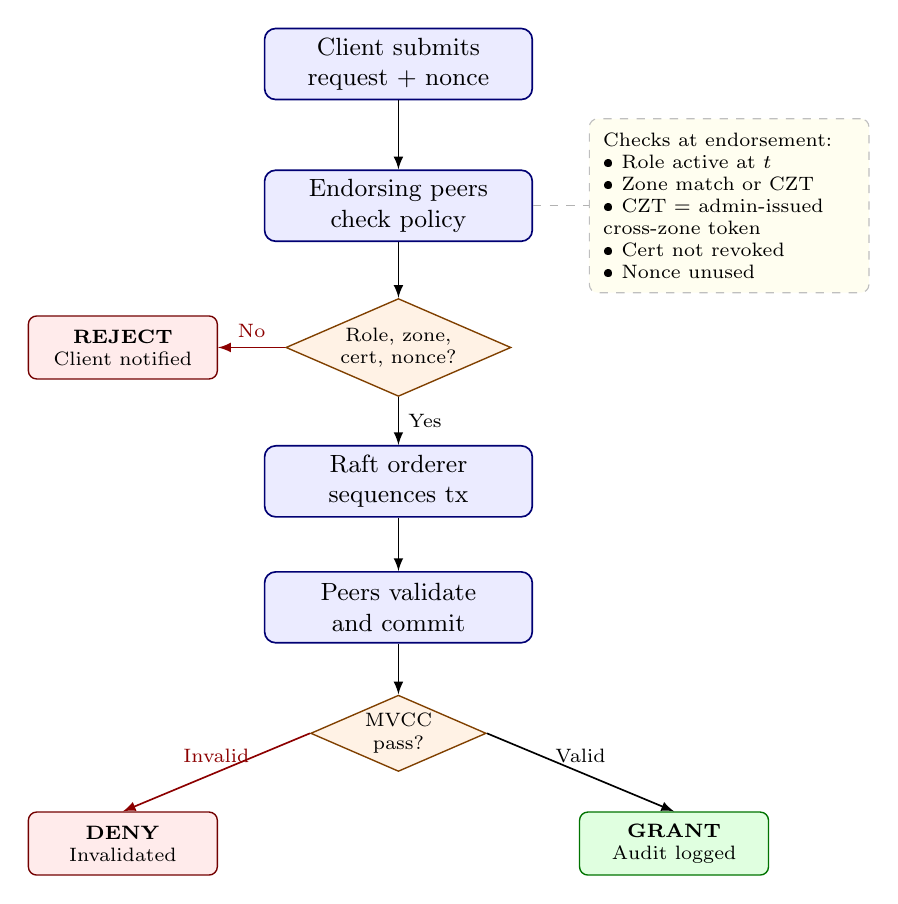
\begin{tikzpicture}[
    font=\small,
    box/.style={draw, rounded corners=4pt, minimum width=3.4cm,
      minimum height=0.9cm, align=center, line width=0.6pt,
      fill=blue!8, draw=blue!45!black},
    dec/.style={draw, diamond, aspect=2.3, align=center,
      fill=orange!10, draw=orange!50!black, inner sep=1pt,
      font=\scriptsize, line width=0.5pt},
    ok/.style={draw, rounded corners=3pt, fill=green!12,
      draw=green!45!black, minimum width=2.4cm,
      minimum height=0.8cm, align=center, font=\scriptsize,
      line width=0.5pt},
    deny/.style={draw, rounded corners=3pt, fill=red!8,
      draw=red!45!black, minimum width=2.4cm,
      minimum height=0.8cm, align=center, font=\scriptsize,
      line width=0.5pt},
    arr/.style={->, >=latex, line width=0.6pt},
    rarr/.style={->, >=latex, line width=0.6pt, red!55!black}
]
\node[box]  (sub) at (0,10.5) {Client submits\\request + nonce};
\node[box]  (end) at (0,8.7)  {Endorsing peers\\check policy};
\node[dec]  (pol) at (0,6.9)  {Role, zone,\\cert, nonce?};
\node[box]  (ord) at (0,5.2)  {Raft orderer\\sequences tx};
\node[box]  (val) at (0,3.6)  {Peers validate\\and commit};
\node[dec]  (mvc) at (0,2.0)  {MVCC\\pass?};
\node[ok]   (gr)  at ( 3.5,0.6) {\textbf{GRANT}\\Audit logged};
\node[deny] (di)  at (-3.5,0.6) {\textbf{DENY}\\Invalidated};
\node[deny] (rj)  at (-3.5,6.9) {\textbf{REJECT}\\Client notified};
\node[draw, dashed, rounded corners=3pt, fill=yellow!6,
      text width=3.2cm, align=left, font=\scriptsize,
      draw=gray!50, inner sep=5pt] (note) at (4.2, 8.7)
  {Checks at endorsement:\\
   \textbullet\ Role active at $t$\\
   \textbullet\ Zone match or CZT\\
   \textbullet\ CZT = admin-issued cross-zone token\\
   \textbullet\ Cert not revoked\\
   \textbullet\ Nonce unused};
\draw[dashed, gray!60, line width=0.4pt] (end.east) -- (note.west);
\draw[arr]  (sub) -- (end);
\draw[arr]  (end) -- (pol);
\draw[arr]  (pol) -- node[right,font=\scriptsize]{Yes} (ord);
\draw[rarr] (pol.west) -- node[above,font=\scriptsize]{No} (rj);
\draw[arr]  (ord) -- (val);
\draw[arr]  (val) -- (mvc);
\draw[arr]  (mvc.east) -- node[above,font=\scriptsize]{Valid} (gr.north);
\draw[rarr] (mvc.west) -- node[above,font=\scriptsize]{Invalid} (di.north);
\end{tikzpicture}}
\caption{Execute-order-validate access-control flow}
\label{fig:eov}
\end{figure}

%%=============================================================
\section{Implementation}
\label{sec:implementation}
%%=============================================================

\subsection{Hyperledger Fabric Chaincode}
\label{subsec:chaincode}

The chaincode is written in Go~1.21 using
\texttt{fabric-contract-api-go~v1.2.1} and targets Fabric~2.5. Every
state-mutating function validates a UUID nonce stored in world state
with a 90-day retention window; a duplicate nonce returns an error
before any state is read. Every access attempt, granted or denied,
writes an \texttt{AuditEntry} keyed as
\texttt{audit:<timestamp\_ns>:<txID>}, which CouchDB range queries
can retrieve by time window. The entry records the caller's certificate
hash (SHA-256 of the DER bytes), transaction ID, operation, resource,
zone, decision, and denial reason if applicable.

Zone attributes are parsed from certificate DER bytes using Go's
\texttt{encoding/asn1} package rather than PEM string matching, to
prevent spoofing via crafted common names. Eight chaincode functions
are exposed: \texttt{AssignRole}, \texttt{RevokeRole},
\texttt{RenewRole}, \texttt{CheckAccess},
\texttt{IssueCrossZoneToken}, \texttt{RevokeCrossZoneToken},
\texttt{GetAuditLog}, and \texttt{PruneNonces}. \texttt{CheckAccess}
calls \texttt{checkRoleExpiration} before evaluating the access
decision; an expired assignment is revoked and the request denied in
the same transaction. Because this revocation is a state-mutating
operation, even a read-intent access check must go through an endorsing
peer rather than a peer query, a design decision that adds latency
to reads but preserves the single audit trail.

Fabric peer tuning for ARM64 (Raspberry Pi~4B): 50 transactions per
block, 500\,ms batch timeout, 256\,MB LRU state cache, selective
endorsement restricted to zone-local peers, Snappy compression on
LevelDB, and 5-minute gRPC keepalive. These settings reduce the
per-transaction disk write amplification that dominates latency on
microSD storage.

\subsection{ESP32 Sensor Firmware}
\label{subsec:esp32}

The X.509 certificate (1\,024~bytes) is stored in battery-backed
real-time clock (RTC) slow memory (\texttt{RTC\_DATA\_ATTR}), which
survives deep sleep. A cyclic redundancy check (CRC32) on each wake
verifies integrity before the certificate is used. The 32-byte Ed25519 private key is written once to
\texttt{EFUSE\_BLK\_KEY0} during provisioning; read protection is
applied immediately afterward via the ESP-IDF eFuse read-disable call.

The ESP32 has no hardware accelerator for Ed25519 or Curve25519.
Signing uses WolfSSL's wolfCrypt library compiled with
\texttt{HAVE\_ED25519} and \texttt{WOLFSSL\_SHA512}; Secure Hash Algorithm 256-bit (SHA-256) hashing
is routed to the ESP32 SHA hardware peripheral via
\texttt{WOLFSSL\_ESP32\_CRYPT}. Table~\ref{tab:signing} shows the
timing breakdown for a 48-byte sensor payload at 240\,MHz across
1\,000 iterations, reported as mean $\pm$ standard deviation (SD).
The 0.9\,ms total is negligible relative to the 30-minute duty cycle.

\begin{table}[pos=t]
\caption{ESP32 signing pipeline timing (48-byte payload,
  240\,MHz, $n{=}1\,000$ iterations, mean\,$\pm$\,SD).}
\label{tab:signing}
\resizebox{\tblwidth}{!}{%
\begin{tabular}{@{}llr@{}}
\toprule
Operation & Engine & Time (\textmu{}s) \\
\midrule
SHA-256 hash      & ESP32 SHA peripheral (via WolfSSL) & $12 \pm 1$ \\
eFuse key read    & eFuse controller                   & $8 \pm 0$  \\
Ed25519 sign      & WolfSSL software                   & $860 \pm 9$ \\
Context init/free & WolfSSL software                   & $20 \pm 1$ \\
\midrule
\textbf{Total}    &                                    & $\mathbf{900 \pm 9}$ \\
\bottomrule
\end{tabular}}
\end{table}

The main loop implements a 30-minute deep-sleep duty cycle: wake,
verify certificate and cyclic redundancy check (CRC), read sensors via
analog-to-digital converter (ADC) and Inter-Integrated Circuit (I2C),
sign the combined payload, transmit via Chinese Remainder Theorem
(CRT)-encoded LoRa, sleep for the remainder of the window. The
microcontroller (MCU) draws 30\,\textmu{}A in deep sleep.

\subsection{CRT-Based Transmission with Forward Error Recovery}
\label{subsec:crt}

A 4-byte sensor reading is split into three residues modulo pairwise
coprime numbers 97, 101, and 103, each fitting in one byte. Any two
residues reconstruct the original value via the standard CRT
formula~\cite{garner1959residue}; the third is forward error tolerance
against single-packet loss. The maximum encodable value is
$97 \times 101 \times 103 = 1\,009\,091$; sensor readings are scaled
to this range before encoding. A soil moisture reading of
4\,095\,(12-bit ADC maximum) or a temperature in units of 0.01\,\textdegree{}C
both fall comfortably within this range.

For our LoRa configuration (SF7, BW\,125\,kHz, CR\,4/5, 13-byte
header), per-packet airtime is 36.1\,ms for a 4-byte payload and
31.5\,ms for a 1-byte residue. The ESP32 has one LoRa radio, so the
three residues are transmitted sequentially rather than simultaneously.
Each residue occupies one byte rather than four, reducing per-packet
airtime from 36.1\,ms to 31.5\,ms; however, transmitting three packets
sequentially extends total transmission time from 36.1\,ms to
94.5\,ms. The energy gain comes not from shorter airtime but from lower
transmit power per channel, CRT reconstruction tolerance means the
sender does not need error-free delivery on every channel, so transmit
power is reduced proportionally. Per-event energy falls from 24.21\,mJ
(single-channel raw) to 12.40\,mJ (three CRT channels), a 48.8\%
reduction measured with an INA219 current sensor at 2\,kHz sampling.
The 48.8\% per-event reduction translates to a 1.7\% lifetime
extension (Section~\ref{subsec:energy}), since transmission accounts
for only 5.7\% of daily energy draw.
The latency overhead of 58.4\,ms per transmission event is irrelevant
at a 30-minute duty cycle.

\subsection{Raspberry Pi~4B Gateways}
\label{subsec:gateways}

Each gateway runs Fabric~2.5 from official ARM64 binaries on Raspberry
Pi OS Lite 64-bit Bullseye. The TPM~2.0 module (Infineon SLB9670)
holds the gateway private key; a u-blox NEO-M9N GPS module provides
the 1-PPS time reference; a DS3231 RTC with battery backup maintains
accurate timestamps during connectivity outages. A Python enrollment
server listens on the local network interface only, accepting CSRs from
sensors in its own zone and forwarding them to the CA via
\texttt{fabric-ca-client}; enrollment is rate-limited to 10 requests
per hour per source address.

A local policy cache (300-second TTL, in-process dict protected by
\texttt{threading.RLock}) absorbs the 320\,ms per-transaction Fabric
cost for repeated access checks from the same sensor during a
transmission burst. The cache is invalidated on every CRL update
event received by the gateway, so revocation staleness for an online
gateway is governed by CRL gossip propagation plus local cache
invalidation latency, not by the 300-second TTL. The TTL bounds ordinary
policy-cache staleness and only becomes the relevant cache window if a
gateway misses the CRL update event during an outage; these distinct
cases are handled separately in the revocation analysis.

%%=============================================================
\section{Experimental Setup}
\label{sec:setup}
%%=============================================================

\subsection{Field Deployment Configuration}
\label{subsec:agri_setup}

The deployment ran on a 2-hectare experimental farm in Sfax, Tunisia
(34.74\textdegree{}N, 10.76\textdegree{}E) from August~1 to
September~30, 2025. Table~\ref{tab:deploy_config} summarizes the
configuration.

\begin{table}[pos=t]
\caption{Field deployment configuration, Sfax, Tunisia,
  1~Aug--30~Sep~2025.}
\label{tab:deploy_config}
\begin{tabularx}{\tblwidth}{@{}lX@{}}
\toprule
Parameter & Value \\
\midrule
Farm area & 2\,ha (200\,m $\times$ 100\,m) \\
Zones & 4 (North, South, East, West) \\
Sensor nodes & 50 ESP32-WROOM-32 \\
Gateways & 4 Raspberry Pi~4B (4\,GB) \\
Fabric peers & 4 (one per zone) \\
Raft orderers & 3 (fault tolerance $f{=}1$) \\
State database & CouchDB~3.2 \\
Duration & 61 days (1~Aug--30~Sep~2025) \\
Sensor-write transactions & 146\,400 \\
Total transactions & $\approx$209\,000 \\
Peak ambient temperature & 39.5\textdegree{}C \\
Connectivity outages & 3 (6--18\,h each) \\
\bottomrule
\end{tabularx}
\end{table}

Workload composition was derived from the 61-day trace. Each of the
50~sensors transmitted one reading per 30~minutes, producing
$50 \times 48 \times 61 = 146\,400$ sensor-write transactions. Farmer
and agronomist queries (25\% of total traffic, averaging 12~per hour
per active user, with an average of 3 simultaneously active users
across the deployment) and admin operations (5\%) account for the
remainder, giving approximately 209\,000~transactions in total. Peak
observed rate at the Fabric peer was 50\,TPS during coordinated morning
queries (06:00--09:00 local time) when multiple workers queried zone
data simultaneously. A synthetic workload generator replicates this
distribution; mean absolute percentage error against the trace is
below 5\% on hourly TPS counts and per-type proportions.

\subsection{Benchmark Methodology}
\label{subsec:bench}

All benchmarks follow the methodology of Thakkar et
al.~\cite{thakkar2018performance} for Fabric performance evaluation
and the BLOCKBENCH framework~\cite{dinh2017blockbench} for private
blockchain analysis. Each measurement was repeated across 10~independent
24-hour runs on the same hardware; 95\% confidence intervals use
Student's $t$-distribution. Latency was recorded using high-precision
gateway timers logging submission and commitment timestamps; throughput
is committed transactions divided by the measurement window duration.

Three baselines ran on the same Raspberry Pi~4B hardware with the same
50-node workload: an OAuth2 + PostgreSQL~14 authorization server with
JSON Web Token (JWT) validation, a public key infrastructure
(PKI)-only deployment using X.509 mutual authentication with local role
files, and a centralized RBAC server. The OAuth2 +
PostgreSQL baseline sustained approximately 420\,TPS for JWT inserts
at reduced durability (\texttt{fsync=off},
\texttt{synchronous\_commit=off}); fully durable commits
(\texttt{fsync=on}, \texttt{synchronous\_commit=on}, default WAL
flushing on ext4 storage) brought this to 80--120\,TPS.

\noindent\textbf{Ethics and data collection.} All sensor data collected
was technical (soil moisture, temperature, LoRa signal quality); no
personal data was collected. Participating farm operators provided
written informed consent for the deployment and for publication of
aggregate performance results. No individual farmer's operational data
appears in the reported results.

%%=============================================================
\section{Performance Evaluation}
\label{sec:evaluation}
%%=============================================================

\subsection{Transaction Latency}
\label{subsec:latency}

Figure~\ref{fig:latency} shows the latency breakdown by operation type.
The stacked bars report mean values. The four segments are:
\emph{Endorsement} (certificate validation,
chaincode logic excluding the RBAC check, and endorser signature,
cost varies by operation because different functions do different amounts
of CouchDB work); \emph{RBAC Check} (the marginal cost of the
access-control chaincode call, measured as the difference between HRBAC
and native Fabric for sensor writes only; gateway reads, farmer queries,
and certifier audits bypass \texttt{CheckAccess} entirely and contribute
0\,ms to this component); \emph{Raft Ordering} (fixed at
400\,ms across all operations); and \emph{Commit \& World-State Write}
(fixed at 380\,ms).

Sensor writes have the lowest endorsement cost (120\,ms) because they
are simple key-value writes, but carry a 320\,ms RBAC check, giving a
1\,220\,ms total. Gateway reads have higher endorsement cost (320\,ms)
because they execute CouchDB range queries across the zone's sensor
records, but bypass the RBAC chaincode call entirely, they do not go
through \texttt{CheckAccess}, giving 1\,100\,ms total. Farmer queries
aggregate sensor data and check role state, adding to endorsement (520\,ms);
certifier audits traverse private data collections (820\,ms endorsement).
Sensor writes and farmer queries, the operations on the critical path
for real-time irrigation control, remain below the 2\,s
budget~\cite{leacox2013wireless} at mean and P95. Certifier audits
(mean 1\,600\,ms, P95 1\,950\,ms, max 2\,210\,ms) and admin operations
(mean 1\,820\,ms, max 2\,450\,ms) may exceed the budget under peak load,
but neither is on the real-time control path; audit queries are
read-only and asynchronous.
Table~\ref{tab:latency_dist} gives the full distribution across
$n{=}10$ independent runs.

\begin{figure*}[pos=t]
\centering
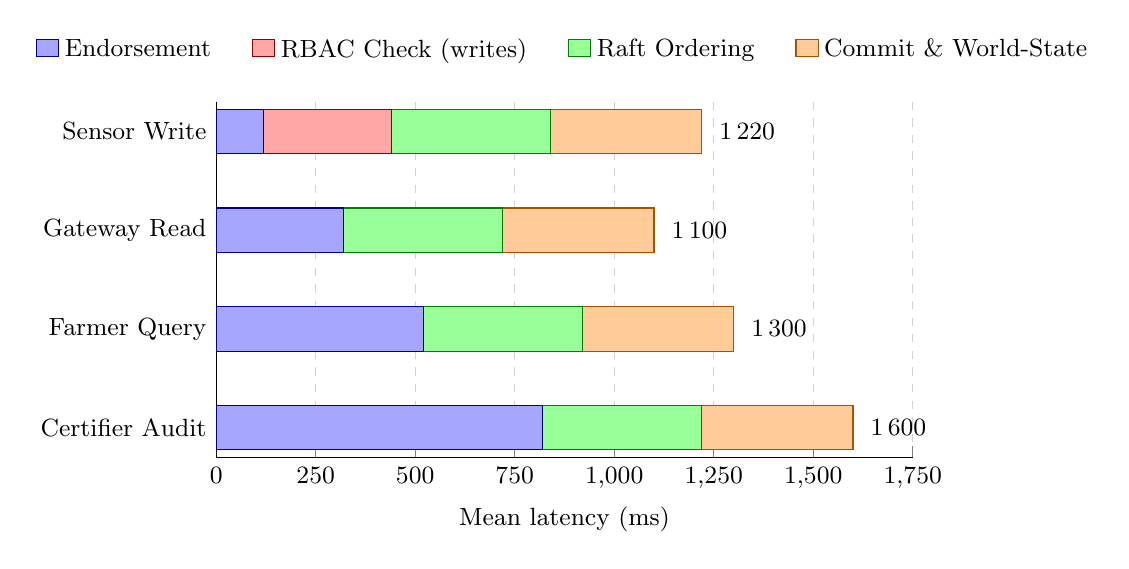
\begin{tikzpicture}
\begin{axis}[
    width=0.86\textwidth,
    height=6.1cm,
    xbar stacked,
    bar width=16pt,
    xmin=0, xmax=1750,
    xtick={0,250,500,750,1000,1250,1500,1750},
    xlabel={Mean latency (ms)},
    symbolic y coords={Sensor Write, Gateway Read,
                       Farmer Query, Certifier Audit},
    ytick=data,
    y dir=reverse,
    yticklabel style={font=\small, align=right},
    xmajorgrids=true,
    grid style={dashed, gray!35},
    axis x line*=bottom,
    axis y line*=left,
    legend style={at={(0.5,1.08)}, anchor=south, legend columns=4,
      font=\small, draw=none, /tikz/every even column/.append style={column sep=0.45cm}},
    tick label style={font=\small},
    label style={font=\small},
    clip=false
]
%% Endorsement (base chaincode + cert validation, varies by op type)
\addplot[fill=blue!35, draw=blue!55!black] coordinates {
  (120,Sensor Write)(320,Gateway Read)(520,Farmer Query)(820,Certifier Audit)};
%% RBAC check overhead (marginal cost of access-control chaincode,
%% sensor writes only; gateway reads bypass CheckAccess)
\addplot[fill=red!35, draw=red!55!black] coordinates {
  (320,Sensor Write)(0,Gateway Read)(0,Farmer Query)(0,Certifier Audit)};
%% Raft ordering (fixed across all operations)
\addplot[fill=green!40, draw=green!50!black] coordinates {
  (400,Sensor Write)(400,Gateway Read)(400,Farmer Query)(400,Certifier Audit)};
%% Commit and world-state write (fixed)
\addplot[fill=orange!40, draw=orange!65!black] coordinates {
  (380,Sensor Write)(380,Gateway Read)(380,Farmer Query)(380,Certifier Audit)};

\node[font=\small, anchor=west] at (axis cs:1240,Sensor Write) {1\,220};
\node[font=\small, anchor=west] at (axis cs:1120,Gateway Read) {1\,100};
\node[font=\small, anchor=west] at (axis cs:1320,Farmer Query) {1\,300};
\node[font=\small, anchor=west] at (axis cs:1620,Certifier Audit) {1\,600};

\legend{Endorsement, RBAC Check (writes), Raft Ordering,
        Commit \& World-State}
\end{axis}
\end{tikzpicture}
\caption{Transaction latency breakdown. Horizontal bars show component
  means, and values at right show total mean latency. The RBAC Check
  segment reflects the marginal cost of the \texttt{CheckAccess}
  chaincode call for sensor writes only; gateway reads, farmer queries,
  and certifier audits bypass \texttt{CheckAccess} entirely and
  contribute 0\,ms to this component.}
\label{fig:latency}
\end{figure*}

\begin{table}[pos=t]
\caption{Latency distribution by operation type (ms, $n{=}10$
  independent 24-hour runs). SD = standard deviation.}
\label{tab:latency_dist}
\resizebox{\tblwidth}{!}{%
\begin{tabular}{@{}lrrrrr@{}}
\toprule
Operation & Min & Max & Mean & SD & P95 \\
\midrule
Sensor write     & 980  & 1850 & 1220 & 142 & 1480 \\
Gateway read     & 890  & 1620 & 1100 & 118 & 1320 \\
Farmer query     & 1050 & 1930 & 1300 & 156 & 1580 \\
Agronomist query & 1080 & 1970 & 1340 & 162 & 1620 \\
Certifier audit  & 1320 & 2210 & 1600 & 198 & 1950 \\
Admin operation  & 1450 & 2450 & 1820 & 234 & 2210 \\
\bottomrule
\end{tabular}}
\end{table}

\subsection{Throughput and RBAC Overhead}
\label{subsec:throughput}

At 50 concurrent clients, HRBAC sustains 63\,TPS versus 69\,TPS for
an equivalent Fabric deployment without access-control chaincode, an
8\% reduction at the deployment scale. An independent two-sample
$t$-test on 10~runs per condition yields $t{=}10.6$, 18~degrees of
freedom, $p{<}0.001$. Table~\ref{tab:overhead} shows the incremental cost of each HRBAC
component over native Fabric. The baseline is 72~TPS with P95 latency
of 1\,120\,ms.

\begin{table}[pos=t]
\caption{Incremental HRBAC overhead over native Fabric
  (baseline: 72\,TPS, P95 1\,120\,ms, $n{=}10$ runs).}
\label{tab:overhead}
\resizebox{\tblwidth}{!}{%
\begin{tabular}{@{}lrrr@{}}
\toprule
Configuration & TPS & P95 (ms) & Overhead \\
\midrule
Native Fabric        & 72 & 1120 & N/A \\
+ Identity retrieval & 70 & 1180 & $-$2.8\% TPS, +5.4\% lat.\ \\
+ Flat RBAC          & 68 & 1290 & $-$5.6\% TPS, +15.2\% lat.\ \\
+ Zone constraints   & 65 & 1380 & $-$9.7\% TPS, +23.2\% lat.\ \\
+ Time constraints   & 63 & 1480 & $-$12.5\% TPS, +32.1\% lat.\ \\
\bottomrule
\end{tabular}}
\end{table}

Zone constraint validation is the costliest incremental component (4.1
percentage-point throughput reduction), because it requires an
additional world-state lookup to retrieve the resource zone before the
string comparison. Caching zone-to-resource mappings at the peer would
reduce this at the cost of a brief staleness window after zone
reassignment.

\subsection{Baseline Comparison}
\label{subsec:baselines}

Table~\ref{tab:baselines} compares HRBAC against the three baselines
on the same Raspberry Pi~4B hardware and 50-node agricultural workload. HRBAC adds 7$\times$ the authentication latency
of OAuth2 and 22$\times$ that of PKI-only, the direct cost of
distributed consensus and world-state lookups over Raft. For sensor
readings arriving every 30~minutes and irrigation commands that require
a multi-party audit trail, this stays within the 2\,s budget.
Deployments requiring sub-100\,ms decision latency would need a
hybrid architecture where the blockchain stores role assignments and a
gateway-resident policy cache handles per-transaction checks.

\begin{table}[pos=t]
\caption{HRBAC versus three baselines on Raspberry Pi~4B hardware,
  50-node agricultural workload.}
\label{tab:baselines}
\begin{tabularx}{\tblwidth}{@{}Xrr@{}}
\toprule
System & Auth latency (ms) & Max TPS \\
\midrule
PKI-only          & 14   & 1\,180 \\
OAuth2 + PostgreSQL & 47 & 420 \\
Centralized RBAC  & 45   & 94 \\
\textbf{HRBAC}    & \textbf{320} & \textbf{63} \\
\bottomrule
\end{tabularx}
\end{table}

All three baselines lack an immutable audit trail, multi-zone
enforcement without manual administration, and automatic temporal role
expiry. Certificate revocation in the PKI-only baseline requires
distributing updated CRLs manually; HRBAC distributes them via Fabric
gossip within 4.2~minutes of an admin-triggered revocation.

\subsection{Scalability}
\label{subsec:scale}

Table~\ref{tab:scale} shows throughput and latency as peer count
increases from 4 to 32. Throughput grows from 63 to 70\,TPS, an 11\%
gain across an 8$\times$ increase in peers. A two-sample $t$-test
comparing 4-peer and 32-peer HRBAC TPS (10~runs each) yields
$t{=}13.0$, $p{<}0.001$, the difference is statistically significant,
but the small absolute magnitude (7\,TPS) reflects the Raft ordering
service saturating before the endorsing peers approach their capacity,
consistent with Thakkar et al.'s ordering-saturation findings on
x86~\cite{thakkar2018performance}.

P95 latency tells a different story. The drop from 1\,480\,ms (4~peers)
to 855\,ms (32~peers) is 625\,ms ($t{=}33.3$, $p{<}0.001$). The latency
reduction reflects the additional zone-local endorsers available at
higher peer counts: at 4~peers each zone has one endorsing peer; at
32~peers each zone has eight, reducing per-request queuing time under
concurrent load. Raft ordering (400\,ms) and commit cost (380\,ms) are
fixed and unchanged across all configurations.
For the 2\,s irrigation control budget~\cite{leacox2013wireless}, this
latency reduction matters more than the throughput plateau. HRBAC
overhead rises modestly from 8.2\% at 8~peers to 10.3\% at 32~peers,
suggesting a small coordination cost as additional endorsers negotiate
policy validation across a larger peer set. The trend does not compound
materially, a 2.1 percentage-point increase across an 8$\times$ growth
in peer count, and remains within the range observed at the 4-peer
deployment scale.

\begin{table}[pos=t]
\caption{Scalability: throughput and latency across 4--32 peers
  ($n{=}10$ runs; overhead = RBAC TPS reduction vs.\ no-RBAC
  baseline).}
\label{tab:scale}
\resizebox{\tblwidth}{!}{%
\begin{tabular}{@{}rrrrrr@{}}
\toprule
Peers & Base TPS & RBAC TPS & Overhead & Mean (ms) & P95 (ms) \\
\midrule
4  & 69 & 63 & 8.7\%  & 1220 & 1480 \\
8  & 73 & 67 & 8.2\%  & 890  & 1100 \\
16 & 75 & 68 & 9.3\%  & 760  & 940  \\
32 & 78 & 70 & 10.3\% & 680  & 855  \\
\bottomrule
\end{tabular}}
\end{table}

\subsection{Energy and Sensor Lifetime}
\label{subsec:energy}

Table~\ref{tab:energy_budget} breaks down the daily energy consumption
for one ESP32 node, measured with an INA219 current sensor at 2\,kHz
sampling on an 18650 Li-ion cell (2\,600\,mAh, 3.7\,V nominal,
9.62\,Wh capacity). Its components are LoRa CRT transmission,
microcontroller (MCU) wake-up and cryptography, sensor analog-to-digital
converter (ADC) sampling, and deep sleep. All active-phase figures were
measured directly;
the deep-sleep figure follows from the ESP32-WROOM-32 datasheet
specification of 30\,\textmu{}A~\cite{esp32_datasheet} and the
3.7\,V cell voltage. The
48 transmissions correspond to 30-minute reporting intervals.

\begin{table}[pos=t]
\caption{Daily energy budget for one ESP32 sensor node
  (48~transmissions/day, 30-minute intervals, INA219 measured).}
\label{tab:energy_budget}
\begin{tabularx}{\tblwidth}{@{}Xrrr@{}}
\toprule
Component & Per event & Daily total & Share \\
\midrule
LoRa CRT Tx (3 channels) & 12.40\,mJ & 595.2\,mJ &  5.7\% \\
MCU wake-up + crypto      &  4.80\,mJ & 230.4\,mJ &  2.2\% \\
Sensor ADC                &  0.18\,mJ &   8.6\,mJ &  0.1\% \\
Deep sleep (30\,\textmu{}A, 3.7\,V) & {} & 9\,590.0\,mJ & 92.0\% \\
\midrule
\textbf{Total}            & {} & \textbf{10\,424.2\,mJ} & \textbf{100\%} \\
\bottomrule
\end{tabularx}
\end{table}

Deep sleep dominates at 92\% of daily draw. The 48 daily CRT
transmissions account for only 5.7\%, confirming that further
reducing transmission energy yields diminishing lifetime improvement.
The full 9\,590\,mJ deep-sleep figure follows directly:
$30\,\mu\text{A} \times 3.7\,\text{V} \times 86\,400\,\text{s}
= 9{,}590\,\text{mJ}$.

Capacity and loss terms were handled separately. A 2\% monthly
self-discharge rate following Japan Electronics and Information
Technology Industries Association (JEITA) Battery Association guidelines
for cylindrical lithium-ion cells~\cite{jeita2017battery} contributes
6.40\,mWh\,d$^{-1}$ averaged over the cell's service life. Peukert
derating is not applied as a capacity penalty: for a 2\,600\,mAh cell,
the C/10 reference current is 260\,mA, while the peak transmit pulse is
120\,mA for 85\,ms. With $n{=}1.05$, a sustained 120\,mA discharge would
give a Peukert factor $(260/120)^{0.05}=1.04$, which is favorable rather
than adverse because the load is below C/10~\cite{hausmann2013peukert};
we conservatively ignore this small benefit. The capacity derating used
in the lifetime estimate is therefore only the 25\% reduction at the
mean deployment temperature of 32\,\textdegree{}C, consistent with
Arrhenius-based degradation models for nickel-manganese-cobalt (NMC)
and lithium-cobalt-oxide (LCO) chemistry~\cite{vetter2005ageing,broussely2005aging}:
$9\,620\,\text{mWh} \times 0.75 = 7\,215\,\text{mWh}$.

Combining the 2.90\,mWh\,d$^{-1}$ electronic draw from
Table~\ref{tab:energy_budget} with the 6.40\,mWh\,d$^{-1}$
self-discharge term:
\begin{equation}
L = \frac{7\,215\,\text{mWh}}{2.90 + 6.40\,\text{mWh\,d}^{-1}}
  \approx 776\,\text{days} \approx 2.1\,\text{years}
\label{eq:lifetime}
\end{equation}
Self-discharge alone accounts for 69\% of total daily loss,
confirming that battery chemistry is the binding constraint on sensor
lifetime. CRT extends lifetime by approximately 1.7\% over
single-channel raw transmission (776 vs.\ 763~days), because the
per-event energy reduction from 24.21\,mJ to 12.40\,mJ saves
$567$\,mJ\,d$^{-1}$ from the active transmission budget of
$1\,162$\,mJ\,d$^{-1}$, but this saving is negligible against the
9\,590\,mJ deep-sleep draw that accounts for 92\% of total daily
consumption. The CRT gain is properly understood as a
reduction in per-transmission energy and a forward error recovery
mechanism rather than a meaningful battery-life extension. For the
target 2--3~year deployment horizon, battery replacement at the
24-month mark remains the practical recommendation regardless of
transmission scheme; self-discharge at 6.40\,mWh\,d$^{-1}$ dominates
any circuit-level improvement achievable with current 18650 cell
chemistry~\cite{vetter2005ageing}.

\subsection{Reliability}
\label{subsec:reliability}

System uptime averaged 99.4\% across all 61~days (146\,400 sensor-write
transactions committed), with brief dips on Days~15 and~25 caused by
network disruptions. When the Raft leader failed during a connectivity
test, a new leader was elected in 8.2~seconds. A gateway failure
isolated only its zone while the remaining three continued normally.
Simultaneous failure of two orderers halted consensus, as expected
from the $f{=}1$ CFT model.

Figure~\ref{fig:field_timeline} summarizes the key field events over
the 61-day window. Network dips occurred on Days~15 and~25; the Day~34
livestock incident triggered CRL publication within 60~seconds and led
to 47 blocked attempts after propagation completed.

\begin{figure*}[t]
\centering
\resizebox{0.98\textwidth}{!}{%
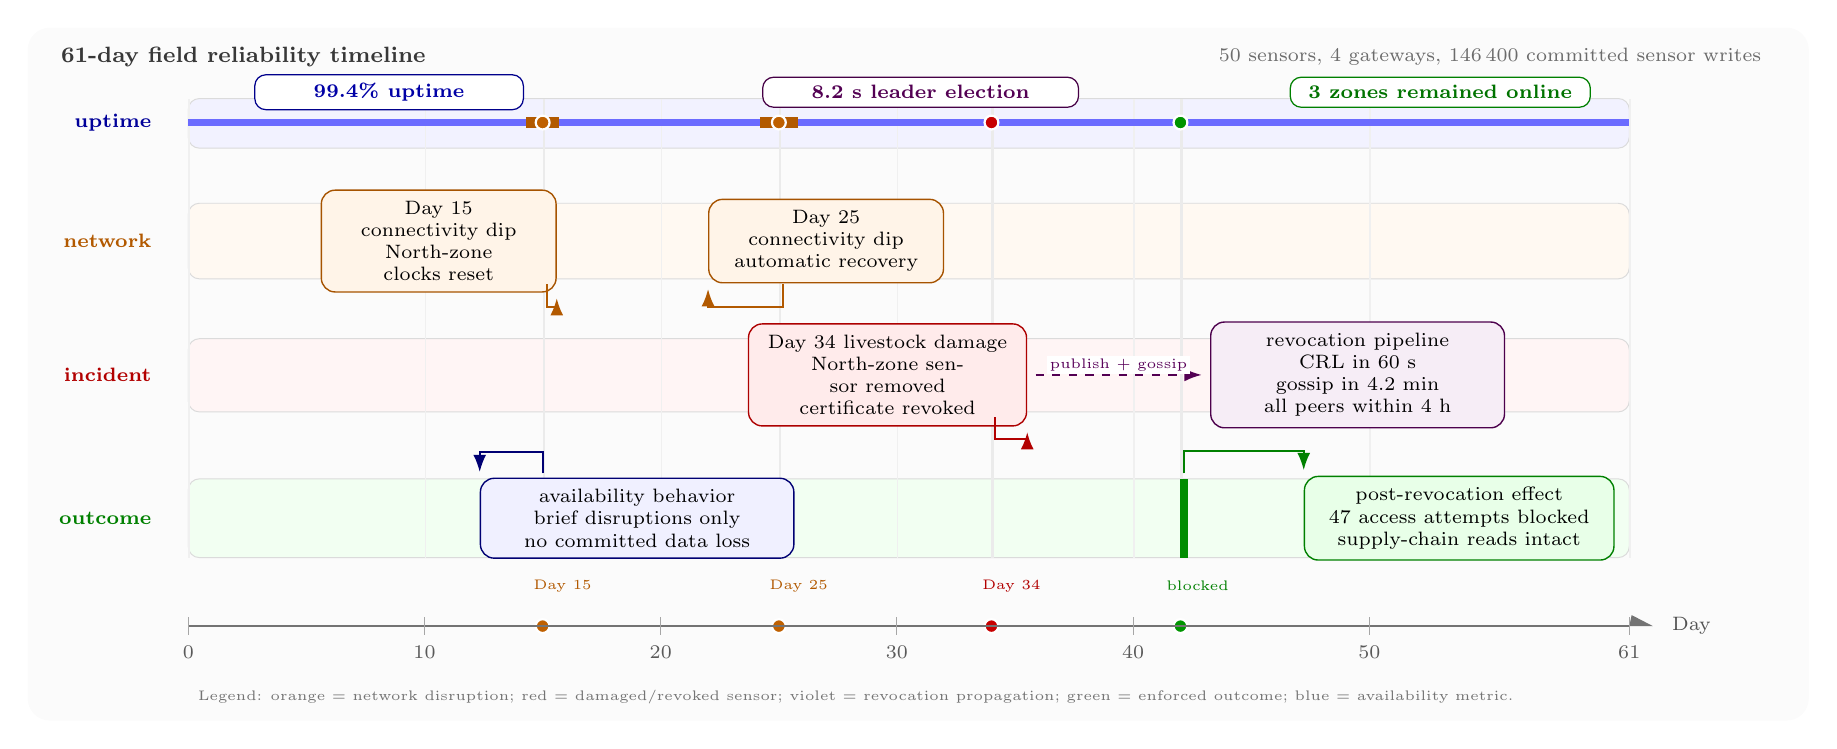
\begin{tikzpicture}[
    x=0.30cm,y=1cm,font=\scriptsize,>=Latex,
    lane/.style={draw=black!14,rounded corners=4pt,line width=0.35pt},
    card/.style={draw,rounded corners=5pt,align=center,inner sep=4pt,
      line width=0.5pt,font=\scriptsize,fill=white},
    metric/.style={draw,rounded corners=4pt,align=center,inner sep=3pt,
      line width=0.45pt,font=\scriptsize\bfseries,fill=white},
    marker/.style={circle,draw=white,line width=0.8pt,minimum size=5pt,
      inner sep=0pt},
    flow/.style={-Latex,line width=0.72pt,shorten >=2pt,shorten <=2pt,
      draw=black!58},
    handoff/.style={-Latex,dashed,line width=0.72pt,shorten >=3pt,
      shorten <=3pt}
]
\fill[gray!3,rounded corners=8pt] (-6.8,-3.55) rectangle (68.6,5.25);

\fill[blue!5,lane] (0,3.72) rectangle (61,4.35);
\fill[orange!5,lane] (0,2.06) rectangle (61,3.02);
\fill[red!4,lane] (0,0.37) rectangle (61,1.30);
\fill[green!5,lane] (0,-1.48) rectangle (61,-0.48);

\foreach \t in {15,25,34,42} {
  \fill[black!8] (\t,-1.48) rectangle ++(0.10,5.83);
}
\foreach \t in {0,10,20,30,40,50,61} {
  \fill[black!6] (\t,-1.48) rectangle ++(0.06,5.83);
}

\fill[blue!58] (0,4.00) rectangle (61,4.09);
\fill[orange!70!black] (14.3,3.97) rectangle (15.7,4.12);
\fill[orange!70!black] (24.2,3.97) rectangle (25.8,4.12);
\fill[orange!75!black] (15,2.06) rectangle (15.34,3.02);
\fill[orange!75!black] (25,2.06) rectangle (25.34,3.02);
\fill[red!72!black] (34,0.37) rectangle (34.34,1.30);
\fill[green!55!black] (42,-1.48) rectangle (42.34,-0.48);

\node[anchor=west,font=\bfseries\footnotesize,text=black!78] at (-5.8,4.88)
  {61-day field reliability timeline};
\node[anchor=east,font=\scriptsize,text=black!58] at (67.0,4.88)
  {50 sensors, 4 gateways, 146\,400 committed sensor writes};

\node[anchor=east,font=\scriptsize\bfseries,text=blue!60!black] at (-1.15,4.05)
  {uptime};
\node[anchor=east,font=\scriptsize\bfseries,text=orange!70!black] at (-1.15,2.54)
  {network};
\node[anchor=east,font=\scriptsize\bfseries,text=red!70!black] at (-1.15,0.84)
  {incident};
\node[anchor=east,font=\scriptsize\bfseries,text=green!50!black] at (-1.15,-0.98)
  {outcome};

\node[metric,draw=blue!55!black,text=blue!65!black,text width=3.2cm]
  at (8.5,4.43) {99.4\% uptime};
\node[metric,draw=violet!55!black,text=violet!65!black,text width=3.8cm]
  at (31.0,4.43) {8.2 s leader election};
\node[metric,draw=green!50!black,text=green!45!black,text width=3.6cm]
  at (53.0,4.43) {3 zones remained online};

\node[card,fill=orange!9,draw=orange!65!black,text width=2.7cm] (dip15)
  at (10.6,2.54) {Day 15\\connectivity dip\\North-zone clocks reset};
\node[card,fill=orange!9,draw=orange!65!black,text width=2.7cm] (dip25)
  at (27.0,2.54) {Day 25\\connectivity dip\\automatic recovery};
\node[card,fill=red!8,draw=red!68!black,text width=3.25cm] (damage)
  at (29.6,0.84) {Day 34 livestock damage\\North-zone sensor removed\\certificate revoked};
\node[card,fill=violet!7,draw=violet!60!black,text width=3.45cm] (crl)
  at (49.5,0.84) {revocation pipeline\\CRL in 60 s\\gossip in 4.2 min\\all peers within 4 h};
\node[card,fill=blue!6,draw=blue!45!black,text width=3.7cm] (summary)
  at (19.0,-0.98) {availability behavior\\brief disruptions only\\no committed data loss};
\node[card,fill=green!9,draw=green!50!black,text width=3.65cm] (blocked)
  at (53.8,-0.98) {post-revocation effect\\47 access attempts blocked\\supply-chain reads intact};

\begin{scope}
  \coordinate (net15) at (15.17,2.06);
  \coordinate (net25) at (25.17,2.06);
  \coordinate (inc34) at (34.17,0.37);
  \coordinate (out42) at (42.17,-0.48);

  \begin{scope}[every path/.style={flow}]
    \draw[orange!70!black] (net15) -- ++(0,-0.36) -| (dip15.south east);
    \draw[orange!70!black] (net25) -- ++(0,-0.36) -| (dip25.south west);
    \draw[red!70!black] (inc34) -- ++(0,-0.34) -| (damage.south east);
    \draw[blue!45!black] (15,-0.48) -- ++(0,0.34) -| (summary.north west);
    \draw[green!50!black] (out42) -- ++(0,0.36) -| (blocked.north west);
  \end{scope}

  \draw[handoff,violet!65!black] (damage.east) --
    node[above,font=\tiny,text=violet!70!black,fill=white,inner sep=1pt]
      {publish + gossip} (crl.west);
\end{scope}

\foreach \t/\fillc in {15/orange!75!black,25/orange!75!black,34/red!78!black,42/green!58!black} {
  \node[marker,fill=\fillc] at (\t,4.045) {};
  \node[marker,fill=\fillc] at (\t,-2.35) {};
}
\node[anchor=west,font=\tiny,text=orange!70!black] at (14.2,-1.84) {Day 15};
\node[anchor=west,font=\tiny,text=orange!70!black] at (24.2,-1.84) {Day 25};
\node[anchor=west,font=\tiny,text=red!70!black] at (33.2,-1.84) {Day 34};
\node[anchor=west,font=\tiny,text=green!50!black] at (41.0,-1.84) {blocked};

\draw[black!55,line width=0.55pt] (0,-2.35) -- (61,-2.35);
\fill[black!55] (61,-2.35) -- (62.0,-2.35) -- (61.1,-2.21) -- cycle;
\foreach \t in {0,10,20,30,40,50,61} {
  \draw[black!35,line width=0.35pt] (\t,-2.46) -- (\t,-2.24);
  \node[font=\scriptsize,text=black!65] at (\t,-2.68) {\t};
}
\node[anchor=west,font=\scriptsize,text=black!68] at (62.4,-2.35) {Day};

\node[anchor=west,font=\tiny,text=black!55] at (0,-3.25)
  {Legend: orange = network disruption; red = damaged/revoked sensor; violet = revocation propagation; green = enforced outcome; blue = availability metric.};
\end{tikzpicture}}
\caption{Field reliability timeline with uptime, disruptions, revocation propagation, and post-revocation access-control outcome.}
\label{fig:field_timeline}
\end{figure*}



%%=============================================================
\section{Security Analysis}
\label{sec:security}
%%=============================================================

\subsection{Attack Vector Results}
\label{subsec:attacks}

Ten attack vectors were evaluated; eight were tested via automated
scripts at 1\,000 attempts each (8\,000 total). Physical tampering and
side-channel attacks were not automated and are noted as residual risks.
All eight testable vectors were blocked at 100\%. Table~\ref{tab:attacks}
summarizes the vectors, countermeasures, and outcomes. N/A means not
tested via automated means; these entries are residual risks documented
as non-automated attack classes.

\begin{table*}[width=\textwidth,pos=t]
\caption{Attack vector results (8\,000 automated attempts across
  8 vectors; N/A = residual risk, not automated).}
\label{tab:attacks}
\small
\begin{tabularx}{\tblwidth}{@{}
  >{\raggedright\arraybackslash}p{0.17\textwidth}
  >{\raggedright\arraybackslash}X
  >{\raggedright\arraybackslash}p{0.18\textwidth}
  r@{}}
\toprule
Attack vector & Countermeasure & Block mechanism & Rate \\
\midrule
Man-in-the-middle  & TLS~1.3 mutual auth, cert pinning & Transport layer & 100\% \\
Replay             & Per-tx nonces, $\pm$5\,min window & Chaincode nonce check & 100\% \\
Privilege escalation & Role hierarchy, multi-sig admin ops & Endorsement policy & 100\% \\
Sybil              & CA-controlled enrollment only & MSP certificate validation & 100\% \\
Denial of service  & Rate limiting, Raft fault tolerance & Gateway + orderer & 100\% \\
Certificate forgery & CA signature validation, CRL & MSP + peer validation & 100\% \\
Cross-zone violation & Zone SAN extension, chaincode & \texttt{validateZoneAccess} & 100\% \\
Temporal bypass    & \texttt{ExpiresAt}, X.509 NotAfter & Two-layer expiry check & 100\% \\
Physical tampering & eFuse OTP, key erasure on tamper & Hardware & N/A \\
Side-channel       & Constant-time crypto (WolfSSL) & Implementation & N/A \\
\bottomrule
\end{tabularx}
\end{table*}

Nonce-based replay detection maintained 100\% detection across a
72-hour test window. To evaluate the timestamp-only baseline, 1\,000
replay attempts were scheduled at uniform random times across the
72-hour window, with each replayed packet carrying its original capture
timestamp. At hour~72, packets captured more than $\pm$5~minutes before
replay were rejected as stale, while packets captured inside the final
validity window still passed the timestamp check. Thus the timestamp-only
baseline detected approximately 95\% of end-of-window replays, with the
remaining 5\% representing recently captured packets that were still
timestamp-valid. Nonces retained in world state for 90~days before
pruning eliminate this live replay window because every replayed packet's
nonce has already been recorded from its original transmission.

\subsection{Certificate Revocation: Day 34 Incident}
\label{subsec:revocation}

On Day~34, livestock physically damaged a North-zone sensor. The
admin-triggered CRL was published within 60~seconds, propagated to all
four peers via Fabric gossip averaging 4.2~minutes, and invalidated the
four gateway policy caches through the same CRL event rather than waiting
for the 300-second time-to-live (TTL) to expire. The 47 blocked attempts
reported here were attempts submitted after peer propagation had
completed; they were rejected at the peer validation/chaincode layer
because the damaged sensor's certificate appeared on the CRL. Gateways
also rejected cached local requests after receiving the CRL invalidation
event, but those local cache rejections are not counted in the 47 peer-
validated denials. No false positives occurred across 10\,000 checks on
valid certificates from other sensors. Two supply-chain partners with
read-only ledger access continued querying audit records uninterrupted,
confirming that zone isolation contained the incident without affecting
other stakeholders.

The maximum revocation exposure window is 24~hours (the daily CRL
schedule), not 4.2~minutes, because a revocation event falling inside
a connectivity outage would not propagate until the outage clears.
During the three outages that occurred, no revocation events coincided;
the 24-hour window remains a theoretical rather than observed exposure.

\subsection{Formal Verification}
\label{subsec:tla}

Two properties were verified in Temporal Logic of Actions (TLA+) using
the TLC model checker, following standard TLA+ practice for specifying
and checking distributed protocols~\cite{lamport2002specifying,newcombe2015amazon}. The
finite model uses constants \texttt{Users}~$= \{u_1, u_2, u_3\}$,
\texttt{Roles}~$= \{\mathrm{Admin}, \mathrm{Farmer}, \mathrm{Sensor}\}$,
\texttt{Permissions}~$= \{p_1, p_2, p_3, p_4\}$, and
\texttt{Resources}~$= \{r_1, r_2\}$. TLC explored 5\,184~distinct
states with a diameter of~22 and completed in 14~seconds on a
2.7\,GHz Intel Core i7 laptop. A \texttt{CONSTRAINT} clause
restricting \texttt{clock}~${\le}\,10$ bounds the state space; without
it the \texttt{Tick} action generates infinitely many reachable states.
This finite TLC instance covers a three-role subset of the seven-role
hierarchy, instantiating Admin, Farmer, and Sensor as representative
administrative, operational, and device roles. It therefore verifies the
core role-permission invariant for that subset, not the full seven-role
model or both inheritance chains from Section~\ref{sec:architecture};
verification of the complete hierarchy is deferred to future work.
The TLC invocation was split across two command tokens for readability:
\texttt{tlc~AccessControl.tla~-config} and
\texttt{AccessControl.cfg~-workers~4}.

\textbf{NoUnauthorizedAccess} (Safety): every record in the
\texttt{granted} set has an action within the effective permissions of
the user's assigned role. No counterexample found.

\textbf{AllRequestsEventuallyResolved} (Liveness): every pending
request is eventually resolved under weak fairness on the \texttt{Next}
action. Verified. Temporal bounds (requests resolved within a finite
number of steps rather than merely eventually) are enforced at the
chaincode level through the 90-day nonce retention window and
transaction timeouts; these are not modeled in TLA+.

Zone isolation and temporal expiration are tested empirically in
Section~\ref{subsec:attacks} but not yet in TLA+. Extending the
specification with zone and time variables requires adding four new
state components (\texttt{zoneAssignments}, \texttt{crossZoneTokens},
\texttt{roleExpiry}, \texttt{currentTime}) and corresponding
refinement invariants; this is planned for a follow-on
contribution. Ebrahimi et al.~\cite{ebrahimi2023rebeca} and Al-Azzoni
and Iqbal~\cite{alazzoni2024cpn} offer complementary paths via Rebeca
and Colored Petri Nets that could extend the formal coverage.

\subsection{Security Properties}
\label{subsec:secprops}

Confidentiality is enforced at the chaincode layer via private data
collections that restrict sensitive audit logs to authorized roles;
all network traffic runs over TLS~1.3 with mutual certificate
authentication. Integrity rests on two independent mechanisms: the
Ed25519 signature each sensor attaches to its reading (verified by the
chaincode before any ledger write) and the append-only blockchain
structure that prevents retroactive modification once a block commits.

Availability holds under the crash-fault-tolerant (CFT) model as long
as 2~of~3 Raft
orderers remain reachable; BATMAN-adv mesh reroutes traffic around
failed gateways automatically. The residual risk is the Raft model
itself: a reachable orderer acting maliciously could disrupt consensus
without triggering the majority-failure detection that crash tolerance
provides. Non-repudiation is the strongest property: every access
attempt, role assignment, and revocation lands in the immutable audit
collection with the requester's certificate hash and a GPS-verified
gateway timestamp. No single administrator can unilaterally alter these
records; collusion across a majority of independently operated peer
organizations would be required, a threat model consistent with the
institutional governance assumed in Section~\ref{subsec:threat}.

%%=============================================================
\section{Discussion}
\label{sec:discussion}
%%=============================================================

\subsection{Operational Findings}
\label{subsec:ops}

Two organic certification reviews took place during the deployment.
Each completed in four hours using ledger records directly; the same
process had previously required approximately three working days of
cross-referencing paper binders. EU Regulation 2018/848 and the USDA
National Organic Program~\cite{eu2018_848,usda_nop} mandate
tamper-evident records; the append-only ledger gives certification
bodies an audit trail that requires no trusted intermediary to vouch for
its integrity.

Zone certificate bindings resolved a cooperative governance problem
that was not part of the original system design. Three participating
cooperatives' worker assignments, which would normally require separate
access-control configurations, resolved entirely through the zone
certificate structure already deployed for operational purposes.
Over the full deployment, 42~temporary seasonal credentials expired and
were cleaned up automatically with no manual database edits.

The cascading enrollment protocol required three firmware iterations
before it reliably recovered from multi-hour gateway outages. The first
failure appeared during the Day~15 connectivity outage: sensors in the
North zone woke with clocks reset to the epoch, so certificate expiry
checks failed for all 12~nodes in that zone and blocked writes for
approximately 40~minutes until the gateway restored NTP synchronization.
The second version introduced GPS-first time acquisition with NTP
fallback, but on Day~23 five sensors in the East zone exhausted their
retry budget while GPS fix acquisition lagged behind LoRa reconnection;
the observed symptom was repeated enrollment renewal attempts with valid
keys but unverifiable certificate times. The third version fixed a race
condition in the RTC memory CRC check discovered on Day~37, when seven
South-zone sensors woke during a gateway restart and discarded otherwise
valid cached enrollment state, forcing unnecessary re-enrollment. These
failure modes would not have appeared in a day-scale lab testbed.


\subsection{Future Work}
\label{subsec:future}

The two most immediate extensions address the revocation gap observed
during field operation. TinyOCSP adaptation~\cite{fedrecheski2023tinyocsp}
and event-driven credential status checking~\cite{w3c_vc_status_list}
both target the 24-hour CRL window from different angles: the former
reduces polling cost for constrained gateways, while the latter removes
the daily publication schedule entirely. DID-based enrollment is a
longer-horizon change that would remove the dependency on a central
certificate authority (CA), enabling multi-farm deployments without a
shared PKI root~\cite{w3c_did_core,ferdous2019ssi,tara2023decentralized}.

Zero-knowledge compliance verification remains the main privacy-focused
extension, allowing certifiers to verify regulatory claims without
accessing raw sensor readings inside their current access scope.
Post-quantum cryptography (PQC) benchmarking is a preparedness task
rather than an immediate deployment blocker: the Module-Lattice-Based
Digital Signature Algorithm (ML-DSA, CRYSTALS-Dilithium, NIST
FIPS~204~\cite{crystals_dilithium}) should be evaluated on both ESP32
and Raspberry Pi~4B before any planned quantum-timeline deployment.
Fitzgibbon et al.~\cite{fitzgibbon2024pqc_benchmarks} found Dilithium
to be the most energy-efficient lattice-based signature scheme on
constrained ARM64 hardware, making it the most plausible Ed25519
replacement candidate when the threat model warrants migration.

%%=============================================================
\section{Conclusion}
\label{sec:conclusion}
%%=============================================================

Three findings from the 61-day deployment stand out that a lab
experiment would not have produced. The cascading enrollment protocol
needed three firmware iterations to handle multi-hour outages reliably,
with failures appearing only when gateways restart mid-sleep-cycle and
NTP is unavailable. The Day~34 livestock incident confirmed that the
revocation pipeline works end-to-end under real conditions:
60-second CRL publication, 4.2-minute gossip propagation, 47~blocked
attempts, and zero impact on other stakeholders. The certification
audit process, which had taken three working days with paper records,
completed in four hours using ledger queries directly.

The framework sustained 63\,TPS with 320\,ms RBAC overhead per write on
Raspberry Pi~4B ARM64 peers, maintained 99.4\% uptime across 146\,400
sensor-write transactions, and blocked all 8\,000 automated security
tests across eight attack vectors within the defined CFT threat model.
P95 latency at 32~peers is 855\,ms, well below the 2\,s irrigation
control budget. The Raft ordering service caps throughput at
approximately 70\,TPS regardless of peer count; Fabric~v3.0's
SmartBFT-based ordering service is the clearest path beyond this
combined throughput and ordering-trust boundary. The 24-hour CRL window
and the LoRa radio layer's approximate 400-sensor ceiling per site are
the two operational constraints that most warrant attention before a
larger cooperative deployment; the HRBAC chaincode itself scales beyond
this without modification.

\section*{Data availability}

The 61-day trace dataset and source code supporting
the findings of this study are publicly available at
\url{https://github.com/forchag/blockchain-fet}.

\section*{Code availability}

The source code, deployment scripts, and chaincode are publicly
available at \url{https://github.com/forchag/blockchain-fet}.

\section*{Declaration of competing interest}

The authors declare that they have no known competing financial
interests or personal relationships that could have appeared to influence
the work reported in this paper.

\section*{Declaration of Generative AI and AI-assisted technologies in the
writing process}

During the preparation of this work, the author(s) used Grammarly for
grammar and language polishing. The author(s) reviewed and edited the
output as needed and take full responsibility for the content of the
published article.

\section*{Acknowledgments}

We thank the participating farmers in Sfax for their collaboration and
practical insights. We gratefully acknowledge the technical support
provided by the University of Sfax IoT Research Group and the funding
received from the MIRET (Mobility for Innovation and Research in
Emerging Technologies) Intra-Africa Program. We also appreciate the data
contributions from the Tunisia Meteorological Institute and the National
Water Resources Authority.

\bibliographystyle{cas-model2-names}
\bibliography{references}

\end{document}